%%%%%%%%%%%%%%%%%%%
\pagebreak
%\cleardoublepage

\columnbreak
\sectionstage[2]{Bilder}

\noindent Tipp: Bei PNG-Bilder immer den transparenten Hintergrund entfernen. Sonst kann es Probleme bei der Darstellung des PDF's geben.

% \negAbstand

\begin{lstlisting}
\usepackage{graphix}	% oder Paket graphics (weniger Möglichkeiten)
\includegraphics[
	width=3cm,			% Breite
	height=3cm,			% Höhe
	keepaspectratio,	% Seitenverh. beh.
	scale=0.5,			% Skalierung
	angle=45				% Winkel in Grad
	trim={links unten rechts oben} % beschneiden (z.B. [0 3cm 0 0])
	clip=true	% true: trim abschneiden; false: trim überstehen lassen
	]{bilder/bild.png} % Bild einbinden

\end{lstlisting}

\negAbstand

% Optionen: fuer includegraphics: angle=, draft, scale=, height=, width=

% ----- Einzelnes Bild -----
\subsectionstage[3]{Einzelnes Bild}
\noindent\begin{minipage}[c]{\linewidth}
	\centering
	
\includegraphics [height=1cm] {Bilder/bild}
	\captionof{figure}[Verzeichniseintrag]{Bildunterschrift}
\end{minipage}

\vspace{-0.5\baselineskip}
\begin{lstlisting}
\begin{figure}[htbp]
	\centering
	
\includegraphics [width=0.8\textwidth] {Bilder/bild.png}
	\caption[Verzeichniseintrag]{Bildunterschrift}
	\label{fig:REFERENZBEZEICHNUNG}
\end{figure}
\end{lstlisting}

\negAbstand
% ----- Bilder nebeneinander -----
\subsectionstage[3]{Bilder nebeneinander} \label{sec:bilder_neben}

\subsubsectionstageS[3]{Gemeinsame Unterschrift}
\noindent\begin{minipage}{\linewidth}
	\centering
	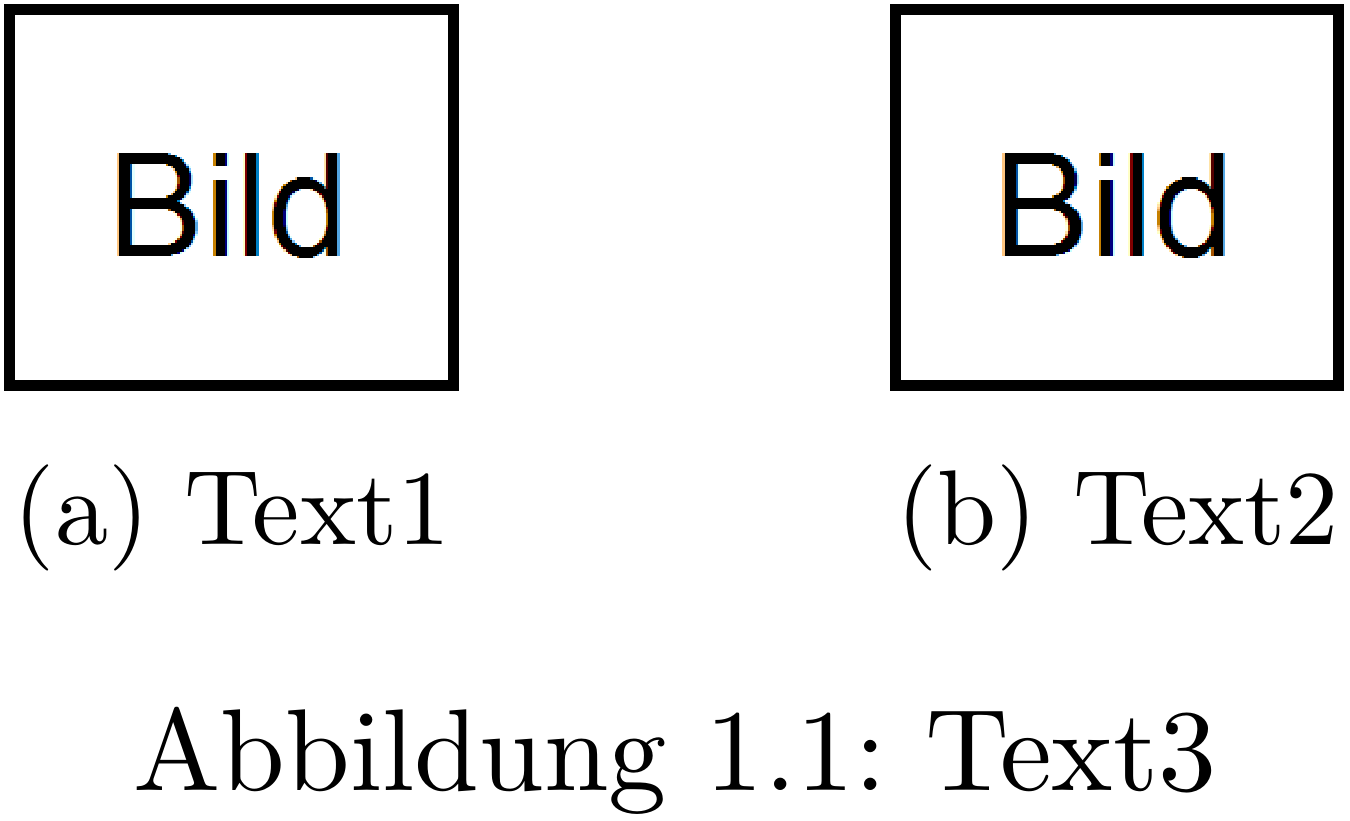
\includegraphics[width=3.5cm,trim={0 7cm 0 0},clip=true]{Bilder/subfigure}
	\captionof{figure}{Text3}
\end{minipage}
%
%
\negAbstand
\begin{lstlisting}
\usepackage{caption,subcaption}
\begin{figure}
\centering
	%
	\begin{subfigure}{0.4\linewidth}
	\centering
		
\includegraphics [width=1.5cm] {Bilder/bild.png}
		\caption{Text1}
	\end{subfigure}
	%
	\begin{subfigure}{0.4\linewidth}
	\centering
		
\includegraphics [width=1.5cm] {Bilder/bild.png}
		\caption{Text2}
	\end{subfigure}
	%
	\caption{Text3}
\end{figure}
\end{lstlisting}



% ----- Eigene Unteschrift -----
\begin{minipage}{\linewidth}
\subsubsectionstageS[3]{Eigene Unterschrift}
%
\begin{minipage}{\linewidth}
		\Centering
	%
	%% Bild Nr. 1
	\begin{minipage}{0.4\linewidth}
		\Centering
    
\includegraphics [width=0.6\linewidth]{Bilder/bild}
		\captionof{figure}{Text}
  \end{minipage}%
	%%
 \hspace{0.1\linewidth}
	%
	%% Bild Nr. 2
  \begin{minipage}{0.4\linewidth}
		\Centering
    
\includegraphics [width=0.6\linewidth]{Bilder/bild}
		\captionof{figure}{Text}
  \end{minipage}
	%
\end{minipage}


% Quellcode:
\vspace{-0.5\baselineskip}
\begin{lstlisting}
\begin{figure}
	\Centering
	\begin{minipage}{0.46\linewidth}
    \Centering
    \includegraphics [width=0.46\linewidth]{Bilder/BILD.png}
		\caption{X}
  \end{minipage}%
	\hspace{1cm}
  %% Bild Nr. 2
  \begin{minipage}{0.46\linewidth}
    \Centering
    \includegraphics [width=0.46\linewidth]{Bilder/BILD.png}
		\caption{X}
  \end{minipage}
\end{figure}
\end{lstlisting}

%%%%%% Quellcode: 
%%%%%\vspace{-0.5\baselineskip}
%%%%%\begin{lstlisting}
%%%%%\begin{figure}{\linewidth}
	%%%%%\Centering
	%%%%%%
	%%%%%\begin{minipage}{0.46\linewidth}
    %%%%%\Centering
    %%%%%\includegraphics [width=1.5cm]{BILD.png}
		%%%%%\captionof{figure}{Bildunterschrift}
  %%%%%\end{minipage}%
  %%%%%%
 %%%%%\hspace{0.5cm}
  %%%%%\begin{minipage}{0.46\linewidth}
    %%%%%\Centering
    %%%%%\includegraphics [width=1.5cm]{BILD.png}
		%%%%%\captionof{figure}{Bildunterschrift}
  %%%%%\end{minipage}
	%%%%%%
%%%%%\end{figure}
%%%%%\end{lstlisting}

\end{minipage}


%%%%%%%%%%%%%%%%%%%%%%%%
\subsectionstage[2]{Textumflossene Bilder}

\begin{multicols}{2}
\begin{wrapfigure}{r}{3cm}
	\centering
	
\includegraphics [width=1cm] {Bilder/bild}
\end{wrapfigure} 
	\bla
%
\columnbreak	
\begin{lstlisting}
\begin{wrapfigure}{r}{3cm}
	\centering
	
\includegraphics [width=1cm] {Bilder/bild.png}
	% \caption[...]{...}
	% \label{fig:...}
\end{wrapfigure} 
\end{lstlisting}
\end{multicols}

\hrule \vspace{0.5\baselineskip}
%----- EOF -----